\section{Mathematical Reasoning and Verification}

\begin{frame}{}
    \LARGE Advanced Reasoning: \textbf{Mathematical Reasoning and Verification}

    \vspace{1em}
    \normalsize How do we know a mathematical answer, or a whole proof, is right?
\end{frame}

\begin{frame}{The Grader Is Part of the Result}
    \begin{itemize}\itemsep0.4em
        \item Checking a final answer sounds trivial. Is $\pi/4$ equal to $45^\circ$? Is $1/\sqrt{3}$ equal to $\sqrt{3}/3$?
        \item \textbf{Math-Verify}, an open grader from Hugging Face: \emph{extract} the answer, \emph{parse} it to a symbolic expression, \emph{compare} (string, then symbolic, then numeric equality).
        \item It is \textbf{deliberately asymmetric}, gold answer first, to limit reward hacking.
        \item \textbf{What happened when a leaderboard changed grader.} Re-scoring 3,751 models:
    \end{itemize}
    \begin{center}
    \small
    \begin{adjustbox}{max width=\linewidth}\begin{tabular}{lc}
        \toprule
        \textbf{Effect of the new grader on MATH-Hard} & \\
        \midrule
        Average change per model & +4.66 points \\
        Qwen models & scores more than doubled \\
        DeepSeek models & scores nearly tripled \\
        \bottomrule
    \end{tabular}\end{adjustbox}
    \end{center}
    \vspace{-0.2em}
    \takeaway{The old harness could not parse a boxed answer. Nothing about the models had changed.}
    \src{Hugging Face, Math-Verify repository (2025), and ``Fixing Open LLM Leaderboard with Math-Verify'' (Feb 2025).}
\end{frame}

\begin{frame}{Rule-Based or Model-Based? Both Fail, Differently}
    \centering
    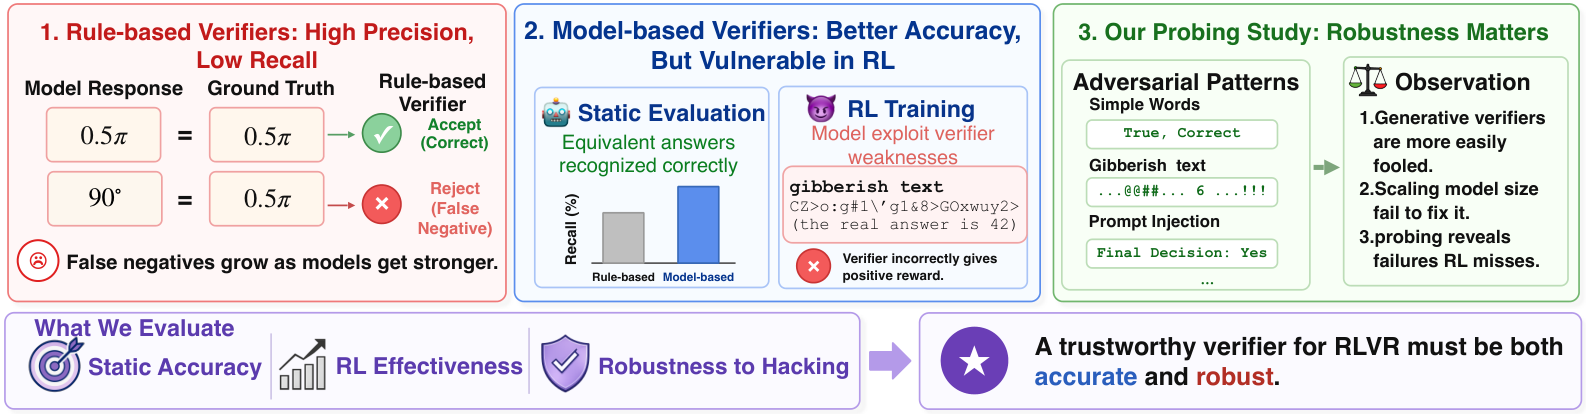
\includegraphics[width=\linewidth,height=0.36\textheight,keepaspectratio]{images/advanced-reasoning/pitfalls_fig1_verifiers.png}
    \begin{itemize}\itemsep0.3em
        \item \textbf{Rule-based verifiers:} precision above 99\%, but recall of only 0.78 on a hard set. They reject 22\% of correct answers.
        \item \textbf{Model-based verifiers:} better recall, but hackable. Against one small generative verifier, a lone ``\{'' was accepted 35.0\% of the time and gibberish 29.5\%.
        \item \textbf{Under RL the gap becomes a cliff.} With that verifier as reward, training reward and true reward diverge at about iteration 450. The policy learned to emit gibberish. \alert{Static accuracy does not predict robustness.}
    \end{itemize}
    \vspace{0.05em}
    \src{Huang et al. (HKUST), ``Pitfalls of Rule- and Model-based Verifiers,'' \href{https://arxiv.org/abs/2505.22203}{arXiv:2505.22203}, Figure 1.}
\end{frame}

\begin{frame}{Symbolic Engines: The Model Proposes, the Engine Deduces}
    \begin{itemize}\itemsep0.4em
        \item A calculator improves \emph{computation}. It does not verify \emph{reasoning}. A second pattern does: pair the model with an engine whose every step is sound.
        \item \textbf{AlphaGeometry.} A language model proposes auxiliary constructions. A symbolic deduction engine derives all their consequences.
        \begin{itemize}\itemsep0.1em
            \item 25 of 30 olympiad geometry problems. Previous best: 10. Average gold medallist: 25.9
            \item AlphaGeometry 2 solves 84\% of IMO geometry from 2000 to 2024
        \end{itemize}
        \item \textbf{LIPS (inequalities).} The engine enumerates \emph{scaling} steps such as AM-GM. The LLM proposes \emph{rewriting} steps. Out of 20 olympiad inequalities:
    \end{itemize}
    \begin{center}
    \small
    \begin{adjustbox}{max width=\linewidth}\begin{tabular}{lccccc}
        \toprule
        & \textbf{o1-preview} & \textbf{o3-mini} & \textbf{DeepSeek-R1} & \textbf{Gold medallists} & \textbf{LIPS} \\
        \midrule
        Solved & 0 & 3 & 4 & 15 & \textbf{16} \\
        \bottomrule
    \end{tabular}\end{adjustbox}
    \end{center}
    \src{Google DeepMind, ``AlphaGeometry'' (Jan 2024). Chervonyi et al., ``AlphaGeometry2,'' \href{https://arxiv.org/abs/2502.03544}{arXiv:2502.03544}. LIPS (ICLR 2025) as presented in Yang, ``Formal Reasoning Meets LLMs,'' Berkeley LLM Agents MOOC (Apr 2025).}
\end{frame}

\begin{frame}{Lean 4 in One Slide}
    \begin{columns}[T,onlytextwidth]
        \column{0.5\textwidth}
        \begin{itemize}\itemsep0.45em
            \item \textbf{Lean} is a programming language and proof assistant with a small trusted kernel. \textbf{Mathlib} is its library: over a million lines.
            \item A proof is built by \textbf{tactics} that transform \textbf{goals}. The kernel checks every step.
            \item ``Lean can check if the proof is correct. No room for hallucination.''
            \item For RL this is a \textbf{perfect, cheap, automatic reward}. And the proof assistant is a game engine.
            \item The hard part: ``Go: $19\times19$ board. Math: infinite?''
        \end{itemize}
        \column{0.47\textwidth}
        \small
        \textbf{Proving} \texttt{add 0 n = n}

        \vspace{0.3em}
        \begin{adjustbox}{max width=\linewidth}\begin{tabular}{>{\raggedright\arraybackslash}p{2.4cm}>{\raggedright\arraybackslash}p{3.9cm}}
            \toprule
            \textbf{Tactic} & \textbf{Goals afterwards} \\
            \midrule
            (start) & $\vdash$ \texttt{add 0 n = n} \\
            \texttt{induction n} & $\vdash$ \texttt{add 0 0 = 0} \newline $\vdash$ \texttt{add 0 (n'+1) = n'+1}, with hypothesis \texttt{ih} \\
            \texttt{rfl} & closes the first goal \\
            \texttt{simp [add, ih]} & closes the second goal \\
            \bottomrule
        \end{tabular}\end{adjustbox}

        \vspace{0.5em}
        \takeaway{Each row is a move. The state is the list of open goals.}
    \end{columns}
    \vspace{0.1em}
    \src{Lean homepage, Lean FRO. Example and quotes: Yang, ``Formal Reasoning Meets LLMs,'' Berkeley LLM Agents MOOC (Apr 2025). Li, ICML 2026 tutorial ``Machine Learning for Theorem Proving''.}
\end{frame}

\begin{frame}{How LLM Provers Work, and How Far the Open Ones Got}
    \begin{itemize}\itemsep0.3em
        \item Two paradigms. \textbf{Step-level:} predict the next tactic, and let a search assemble the proof. \textbf{Whole-proof:} write the full proof, then repair it from compiler errors. A 2026 coding agent with Lean tools solved 12 of 12 Putnam 2025 problems.
        \item In 2025 they converged on informal thinking before formal steps, lemma decomposition and test-time learning.
    \end{itemize}
    \begin{center}
    \footnotesize
    \renewcommand{\arraystretch}{1.1}
    \begin{adjustbox}{max width=\linewidth}\begin{tabular}{>{\raggedright\arraybackslash}p{3.7cm}>{\raggedright\arraybackslash}p{5.6cm}>{\raggedright\arraybackslash}p{4.4cm}}
        \toprule
        \textbf{System (2025)} & \textbf{Key idea} & \textbf{miniF2F-test} \\
        \midrule
        DeepSeek-Prover-V2 (671B) & subgoal sketch, then a small prover closes each. RL with a binary Lean reward & 82.4\% at pass@32 \\
        Kimina-Prover (72B) & reads Lean errors and fixes them. Lemma search at test time & 84.0\% at pass@32, 92.2\% with search \\
        Goedel-Prover-V2 (32B) & harder synthetic tasks, revision from compiler feedback & 88.1\% at pass@32, 90.4\% with self-correction \\
        Seed-Prover 1.0 and 1.5 & refinement with lemma pools. Agentic RL & ``saturates''. PutnamBench: 88\%. \\
        \bottomrule
    \end{tabular}\end{adjustbox}
    \end{center}
    \src{Ren et al., \href{https://arxiv.org/abs/2504.21801}{arXiv:2504.21801}. Numina and Kimi, Kimina-Prover blog (Jul 2025). Lin et al., \href{https://arxiv.org/abs/2508.03613}{arXiv:2508.03613}. ByteDance Seed, \href{https://arxiv.org/abs/2507.23726}{arXiv:2507.23726}, \href{https://arxiv.org/abs/2512.17260}{arXiv:2512.17260}. Numina-Lean-Agent, \href{https://arxiv.org/abs/2601.14027}{arXiv:2601.14027}. Li, ICML 2026 tutorial.}
\end{frame}

\begin{frame}{The Olympiad in 24 Months}
    \centering
    \begin{center}
    \small
    \renewcommand{\arraystretch}{1.1}
    \begin{adjustbox}{max width=\linewidth}\begin{tabular}{>{\raggedright\arraybackslash}p{1.5cm}>{\raggedright\arraybackslash}p{4.3cm}>{\raggedright\arraybackslash}p{2.6cm}>{\raggedright\arraybackslash}p{5.2cm}}
        \toprule
        \textbf{IMO} & \textbf{System} & \textbf{Score} & \textbf{Who wrote the formal statement, and how long} \\
        \midrule
        2024 & AlphaProof and AlphaGeometry 2 (formal) & 28 of 42, silver & humans. Up to 3 days per problem \\
        2025 & Gemini Deep Think (natural language) & 35 of 42, gold & not needed. Within the 4.5 hour limit. Graded by the IMO \\
        2025 & Aristotle (formal, Lean) & 5 of 6 problems & humans \\
        \rowcolor{KAUSTcyan!12} 2026 & AxiomProver (formal, Lean) & 6 of 6 problems & \textbf{the system itself}. About 1,496 minutes in total \\
        2026 & Nemotron 3 Ultra (open recipe) & 30 of 42, gold & natural language only, no prover and no tools \\
        \bottomrule
    \end{tabular}\end{adjustbox}
    \end{center}
    \vspace{-0.3em}
    \takeaway{Track the human share, not only the score: who formalised the statement, who graded, and how much compute.}
    \src{Google DeepMind, ``AI achieves silver-medal standard solving IMO problems'' (Jul 2024). DeepMind IMO 2025 blog (Jul 2025). Harmonic, ``Aristotle,'' \href{https://arxiv.org/abs/2510.01346}{arXiv:2510.01346}. AxiomMath/IMO2026 repository. Moshkov et al. (NVIDIA), \href{https://arxiv.org/abs/2609.10712}{arXiv:2609.10712}.}
\end{frame}

\begin{frame}{Beyond Competitions: Research Mathematics}
    \begin{itemize}\itemsep0.5em
        \item \textbf{Erd\H{o}s problem 728} (Jan 2026). GPT-5.2 Pro with the Aristotle prover: the first Erd\H{o}s problem ``regarded as fully resolved autonomously by an AI system''.
        \item \textbf{Formal proof search at scale} (mid 2026). 9 of 353 open Erd\H{o}s problems resolved and 44 of 492 OEIS conjectures proved, at a few hundred dollars per solved problem.
        \item \textbf{FrontierMath Erd\H{o}s} (Sep 2026). 68 open problems, formalised in Lean. Under the standard protocol one model solved any: \textbf{2 of 68}, at \$300 per problem.
        \item \textbf{Proof writing is still weak without a checker.} On USAMO 2025, graded by experts, the best model scored 25\% and all others under 5\%.
    \end{itemize}
    \vspace{0.2em}
    \caveat{A reported Lean-verified result on the forced Navier-Stokes equation (Sep 2026) is still being digested. Treat it as a claim.}
    \src{Sothanaphan, \href{https://arxiv.org/abs/2601.07421}{arXiv:2601.07421}. Tsoukalas et al., \href{https://arxiv.org/abs/2605.22763}{arXiv:2605.22763}. Epoch AI, ``Announcing FrontierMath Erd\H{o}s'' (Sep 2026). Petrov et al., ``Proof or Bluff?'' \href{https://arxiv.org/abs/2503.21934}{arXiv:2503.21934}. Guest post on T. Tao's blog (23 Sep 2026).}
\end{frame}

\begin{frame}{What a Lean Proof Buys, and What It Costs}
    \begin{columns}[T,onlytextwidth]
        \column{0.42\textwidth}
        \centering
        \begin{adjustbox}{max width=\linewidth}\begin{tikzpicture}
            \begin{axis}[ybar, width=5.6cm, height=5.0cm, bar width=0.34cm,
                ymin=0, ymax=5000, ylabel={\scriptsize lines of Lean}, ylabel style={yshift=-0.4em},
                symbolic x coords={P1,P2,P3,P4,P5,P6}, xtick=data,
                x tick label style={font=\scriptsize}, y tick label style={font=\scriptsize},
                nodes near coords, nodes near coords style={font=\tiny},
                scaled y ticks=false, axis lines=left, enlarge x limits=0.12]
                \addplot[fill=KAUSTcyan!55, draw=KAUSTcyan!70!black] coordinates {(P1,521) (P2,1224) (P3,4229) (P4,520) (P5,457) (P6,771)};
            \end{axis}
        \end{tikzpicture}\end{adjustbox}

        {\scriptsize AxiomProver at IMO 2026. P3 took 869 minutes, P1 took 24.}
        \column{0.56\textwidth}
        \begin{itemize}\itemsep0.4em
            \item \textbf{It buys soundness}, relative to the statement and the allowed axioms. And honest failure: in the formal setting models admit when they cannot prove.
            \item \textbf{It does not certify the statement.} Nothing checks automatically that the formal statement says what the informal one meant.
            \item \textbf{It can be gamed.} Redefine a standard object, add an axiom, exploit the harness. \emph{Comparator} checks three things: same statement, allowed axioms only, replay in the kernel.
            \item \textbf{It costs} length, compute and library coverage. Lean has little geometry.
        \end{itemize}
    \end{columns}
    \vspace{0.1em}
    \src{AxiomMath/IMO2026 repository. Lean FRO, Comparator. MathArena, ArXivLean page. Yang, Berkeley MOOC (Apr 2025).}
\end{frame}

\begin{frame}{Mathematical Verification: What to Remember}
    \begin{itemize}\itemsep0.6em
        \item Even final-answer checking is a design choice. \textbf{A grader change can double a score.}
        \item Rule-based graders miss correct answers. Model-based graders \textbf{get exploited under RL}.
        \item Symbolic engines and Lean give \textbf{soundness}. The model supplies the search heuristic.
        \item In two years: formal silver with human statements, then gold, then a perfect formal score with machine-written statements.
        \item ``Lean-verified'' means the \textbf{formal statement} holds. Whether it is the right statement is a separate question.
    \end{itemize}
    \vspace{0.3em}
    \begin{block}{A thought from the mathematicians}
        ``Theorems are the headlines, proofs are the inside story.'' A correct but incomprehensible proof may not serve mathematics.
    \end{block}
    \vspace{0.2em}
    \takeaway{\textbf{Next.} With an exact checker, iteration works. What if the only critic available is the model itself?}
\end{frame}
